\documentclass[10pt, twoside, a4paper]{article}
\usepackage{fancyhdr}
\usepackage{amsmath, amsthm, amssymb}
\usepackage[catalan]{babel}
\usepackage[titles]{tocloft}
\usepackage[utf8]{inputenc}
\usepackage[left=2.15cm, right=2.15cm, top=30mm, bottom=20mm]{geometry}
\usepackage{parskip}
\usepackage{subcaption}
\usepackage{titlesec}
\usepackage{bookmark}
\usepackage{multirow}
\usepackage{graphicx}
\usepackage{physics}
\usepackage{hyperref}
\usepackage{float}
\usepackage{caption}
\usepackage{booktabs}
\captionsetup{labelfont=bf}

\begin{document}

\begin{titlepage}
\centering
{\LARGE Mètodes Numèrics II \par}
\vspace{2cm}
{\Huge \textbf{Pràctica de simulació:} \par}
\vspace{1cm}
{\Huge \textbf{Modelització del comportoment d'una placa fotovoltaica} \par}
\vspace{3cm}
{\Large G01 \par}
\vspace{0.5cm}
{\Large 1549086: Bujones Umbert, Jun Shan\\1666739: Franco Avilés, Eric\\  1672980: González Barea, Eric\\1644841: Vilarrúbias Morral, Natàlia \par}
\vspace{2cm}
{\Large Gener 2025 \par}
\vspace{2cm}

\includegraphics[width=0.4\textwidth]{Logo_UAB.png}


\end{titlepage}

\pagenumbering{gobble}
\renewcommand{\cftsecfont}{}
\renewcommand{\cftsecpagefont}{}
\renewcommand{\cftsecleader}{\cftdotfill{\cftdotsep}}
\renewcommand{\cftdotsep}{0.2}
\setlength{\cftbeforesecskip}{0.5em}
\setlength{\cftbeforesubsecskip}{0.5em}
\tableofcontents

\newpage
\pagenumbering{arabic}
\setcounter{page}{1}

\pagestyle{fancy}
\lhead{\textbf{Pràctica de Simulació}}
\rhead{\textbf{Mètodes Numèrics II}}

\section{Introducció i Objectius}
Amb el pretext de poder calcular l'energia subministrada per una placa solar de superfície igual a 2 m$^2$ situada en un habitatge unifamiliar de Mont-rós (poble de la província de Lleida, Catalunya), en aquesta pràctica ens plantegem modelitzar el moviment del Sol sobre aquesta localitat en el transcurs de tot un any. 

Per aconseguir això últim, proposem fer una simulació del Sistema Solar usant el mètode d'Euler per a diverses discretitzacions temporals, tenint en compte un seguit d'aproximacions fonamentals, entre les quals en destaquem la consideració que tots els planetes es mouen sobre el pla de l'eclíptica i que el Sistema Solar simulat està conformat pels 5 primer planetes del cas real. En els annexos, però, ampliem aquest estudi considerant un cas més pròxim a la realitat i adjuntant, a més a més, un seguit d'animacions que ens permetran visualitzar millor la dinàmica del sistema caracteritzat. 

\section{Plantejament del problema del Sistema Solar}

\subsection{Modelització del Sistema Solar}
Per tal de modelitzar el Sistema Solar, partirem de la Segona Llei de Newton i la igualarem a la Lley de la Gravitació Universal, tot dividint per la massa del cos $p$, $M_p$. Fent això ens queda que l'acceleració a la qual està sotmesa aquest cos és:

\begin{equation}
    \derivative[2]{\mathbf{r}^{(p)}}{t} = - G \left[ \sum_{l \neq p} M_l \frac{(\mathbf{r}^{(p)}-\mathbf{r}^{(l)})}{\abs{\mathbf{r}^{(p)} - \mathbf{r}^{(l)}}^3}\right], \hspace{0.25cm} p = 1, 2, \ldots 
\end{equation}

En aquesta equació el vector $\mathbf{r}^{(p)}$ és el vector posició (marquem els vectors en negreta) del cos $p$ respecte del Sol (de manera que el nostre origen de coordenades serà la posició inicial del Sol), $M_l$ la massa dels cossos diferents a $p$ i $\mathbf{r}^{(l)}$ les seves posicions respecte l'origen. Fixem-nos, doncs, que segons aquesta equació, la força que actua sobre un planeta donat es correspon amb la suma de les forces exercides per tots els cossos del sistema solar sobre ell. 

Simplificarem l'expressió definint $\mathbf{d}_{pl} \equiv (\mathbf{r}^{(p)}-\mathbf{r}^{(l)})$. Així, la darrera equació queda com
\begin{equation}
    \derivative[2]{\mathbf{r}^{(p)}}{t} = - G \left[ \sum_{l \neq p} M_l \frac{\mathbf{d}_{lp}}{\abs{\mathbf{d}_{lp}}^3}\right], \hspace{0.25cm} p = 1, 2, \ldots 
\end{equation}

Per tal de facilitar-ne la ressolució, podem transformar aquesta equació diferencial de segon ordre a la següent

\begin{equation}
    \derivative{\mathbf{v}^{(p)}}{t} = -G \left[ \sum_{l \neq p} M_l\frac{\mathbf{d}_{lp}}{\abs{\mathbf{d}_{lp}}^3}\right], \hspace{0.25cm} p = 1,2 \ldots \label{2}
\end{equation}

De forma que tenim ara un conjunt de $n \cross p$ (on $n$ són les dimensions) equacions diferencials de primer ordre a resoldre. A la pràctica, com que tots els planetes del sistema solar tenen orbites coplanàries (a excepció de Plutó, que no el considerarem), podem assumir que estem davant d'un problema bidimensional, de manera que tindre $2 \cross p$ EDOs de primer ordre a resoldre.

Considerarem un model en què els únics cossos del Sistema Solar són Mercuri, Venus, la Terra, Mart i Júpiter (i, naturalment, el Sol), per tal de simplificar les gràfiques. A més a més, el moviment d'aquests cossos serà al pla de l'eclíptica; no considerarem moviments en l'eix $z$. Es podrà trobar una versió més complexa (amb la modelització de tots els planetes i les corresponents gràfiques per diferents temps finals) al repositori de \textit{GitHub} (veure annex \ref{an:a}). A l'annex \ref{an:b} donem un breu resum d'això últim en forma de material extra.

\subsection{Normalització de les equacions}
Per tal de resoldre el problema minimitzant errors i temps de càlcul cal normalitzar \eqref{2}. Definim unes quantitats característiques del sistema: escollim $M_0 = M_s$ (la massa del Sol) i $d_0 = UA$ (unitat astronòmica), ja que així podrem treballar amb valors propers a la unitat. D'aquí se'n deriva que
\begin{equation*}
    t_0 = \sqrt{\frac{d_0^3}{M_s \cdot G}}
\end{equation*}
Usant tot això, podem arribar fàcilment a 
\begin{equation}
    \derivative[2]{\mathbf{\tilde{r}}^{(p)}}{\tilde{t}} = - \sum_{l \neq p} \frac{\mathbf{d}_{lp}}{\abs{\mathbf{d}_{lp}}^3}, \hspace{0.25cm} p = 1,2 \ldots
\end{equation}
d'on tenim que
\begin{equation}
    \boxed{\derivative{\tilde{v}_i^{(p)}}{\tilde{t}} = - \sum_{l \neq p} M_l \frac{d_{lp,i}}{\abs{\mathbf{d}_{lp}}^3} \hspace{0.25cm} p = 1,2 \ldots, \hspace{0.25cm} i = 1, 2} \label{eq5}
\end{equation}

\subsection{Condicions inicials}
Per tal de conèixer les condicions inicials de cadascun dels cossos del sistema solar modelitzat (això és, $\mathbf{r}^{(p)}$ i $\mathbf{v}^{(p)}$) hem usat la base de dades del \textit{Horizons Ephemeris Service} de la NASA, que podeu trobar a \url{https://ssd.jpl.nasa.gov/horizons/}. Agafem com a punt inicial les posicions i les velocitats el dia 01-01-2025 de tots els cossos rellevants del sistema solar.

\subsection{Mètode numèric i avaluació de l'error}
El mètode numèric utilitzat ha estat el mètode d'Euler (per sistemes EDOs)\footnote{Les corresponents equacions es poden consultar als apunts de l'assignatura.} aplicat a l'equació \eqref{eq5} per diferents discretitzacions temporals: $dt = 1$ any, $dt = 1$ mes i $dt = 1$ dia.

Per tal d'avaluar l'error comés estudiarem l'evolució d'una de les quantitats conservades d'aquest sistema: L'energia total $\varepsilon$. Idealment, a cada cas d'iteració el valor de $E$ ha de ser el mateix que a $t_0$; les fluctuacions en aquestes quantitats ens permetran determinar l'error numèric comès segons:
\begin{align}
    E_{\varepsilon_i} = \left( \frac{\Delta \varepsilon_i}{\varepsilon_0} \right) & = \frac{\varepsilon_i - \varepsilon_0}{\varepsilon_0} 
\end{align}

On el valor de $\varepsilon$ es pot treure a partir de les equacions fonamentals de la dinàmica.

\section{Plantejament del problema de la placa solar}

\subsection{Modelització del moviment del Sol sobre Mont-rós}
Per modelitzar el moviment del Sol des d'un sistema de referència situat en una teulada a Mont-rós, partim d'unes coordenades esfèriques on un angle $\theta$ indica l'alçada del sol i un angle $\phi$ indica la posició horizontal del sol utilitzant el centre de la placa solar com a origen de coordenades.

Així doncs, partint d'aquests angles, realitzem una discretització de cada angle en funció de les hores de llum solar que té cada dia de l'any\footnote{Informació que hem extret de \url{https://meteogram.es/sol/espana/vielha/}}. En aquesta discretització tenim en compte els angles $\phi$ que limiten la regió on rebem incidència de llum solar i els angles $\theta$ màxims als quals arriba el sol depenent de l'estació de l'any, aquests últims delimitats en un interval determinat per la latitud de Mont-rós $\pm 15^\circ$.

\textbf{(falta imagen de las coordenadas utilizadas)}

\subsection{Modelització de l'electricitat generada per la placa solar}
A partir del model del moviment solar, plantegem els mateixos angles $\theta$ i $\phi$ però escollint com a origen de coordenades el centre de la placa solar; d'aquesta manera podrem definir la incidència lumínica que rebem en cada discretització temporal com $W = W_{max}\cos(\theta)\cos(\phi)$, on $W_{max} = 1000 \text{ W/m$^2$}$. Amb aquesta expressió ja podem calcular l'electricitat generada en tot l'any tenint en compte la variació horària i del moviment solar en les diferents estacions.

Tot seguit presentem el seguit de consideracions extres de caràcter geogràgic i/o metereològic que tindrem en compte en el nostre model. L'estudi climàtic s'ha efectuat amb dades històriques extretes de la web de \textit{Nasa Power}, veure \cite{ref6}.
\begin{itemize}
    \item Mont-rós és una localitat amb un horitzó no pla, ja que està envoltat de muntanyes que limiten les hores de llum diàries. Per tal de tenir present aquest fenomen cal introduir una variació en els angles $\phi$ inicials i finals. Eliminem els angles $\phi < -77$ º i $\phi > 82$ º, en tant que no contribueixen de manera significativa a la irradiació efectiva de les plaques solar. Aquests valors els hem extret estudiant l'alçada relativa al poble de les muntanyes properes a aquestes usant \textit{Google Maps}. 
    \item Les precipitacions lleus no només afecten negativament el rendiment de les plaques fotovoltaiques, sinó que també poden ser beneficioses, netejant, per exemple, la seva superfície. En aquest context, hem considerat que (en promig):
    \begin{itemize}
        \item Les pluges lleus no afecten el rendiment de les plaques.
        \item Les pluges moderades (4-10 mm/h) redueixen el rendiment en un 15\%.
        \item Les pluges intenses ($>$ 10 mm/h) redueixen el rendiment en un 25\%.
    \end{itemize}
    \item Pel que fa a les nevades, segons les dades històriques al poble neva, fonamentalment, entre gener i mitjans de març. Tot i que la neu pot arribar a ser altament perjudicial sobre les plaques (bloquejant completament la llum solar), la inclinació de les plaques (de 42.5 º) redueix considerablement aquest risc, així que es negligirà. A tot això cal afegir que les nevades a la zona són puntuals i de baixa intensitat, fet que facilita el desglaç i que la neu acumulada als voltants de la placa podria crear un efecte reflectant, incrementant així la captació solar.
    En cas necessari es pot instal·lar un sistema antidesglaç o una cobertura hidrofòbica, tot i que aquestes opcions consumirien part de l'energia generada. 
    Tenint en compte tots els factors comentats s'ha aplicat un factor de reducció del 20\% al rendiment durant el període de neu, com a estimació conservadora.
    \item Les plaques fotovoltaiques comencen a perdre, en general, eficiència a temperatures superiors a $T=25$ ºC, reduint-se el rendiment en un 0.3\% inicialment. A Mont-rós les temperatures són generalment baixes, amb un clima fred a causa de la seva altitud. El problema de la temperatura només es presentaria, doncs, a l'estiu, quan les temperatures poden superar, segons els registres històrics, els 25 ºC entre les 12:00 i les 15:00 hores, arribant a màximes de 31 ºC, però en períodes breus. 
    Per tot això, hem considerat que els efectes associats a la temperatura són negligibles sobre el rendiment de la placa fotovoltaica.
\end{itemize}

\textbf{(estaria guay poner una imagen del sistema desde la placa, si se puede)}

\subsection{Avaluació de l'error}
Per tal d'evaluar com d'exacte és el nostre model, els resultats obtinguts es compararan amb els del PVGIS \cite{ref7}. Calcularem l'error relatiu associat a l'energia subministrada per la placa fotovoltaica com:
\begin{equation}
    E_{placa} = \frac{\abs{\varepsilon_{model}-\varepsilon_{teo}}}{\varepsilon_{teo}}\cdot 100
\end{equation}
on $\varepsilon_{model}$ i $\varepsilon_{teo}$ són les energies associades al nostre model i als resultats obtinguts del PVGIS, respectivament.

\section{Resultats i discussió}

\subsection{Sistema Solar}
Després d'implementar el mètode numèric s'han trobat les òrbites (per a cada valor de $dt$) fins a $t=1$ any (terrestre) que es poden veure a la figura \ref{fig1}. Més tard, a la figura \ref{fig4}, podem veure les òrbites per a $t=100$ anys per la discretització $dt=1$ dia amb el corresponent error.
 
\begin{figure}[h]
    \centering
    
    \begin{subfigure}[b]{0.32\linewidth}
        \centering
        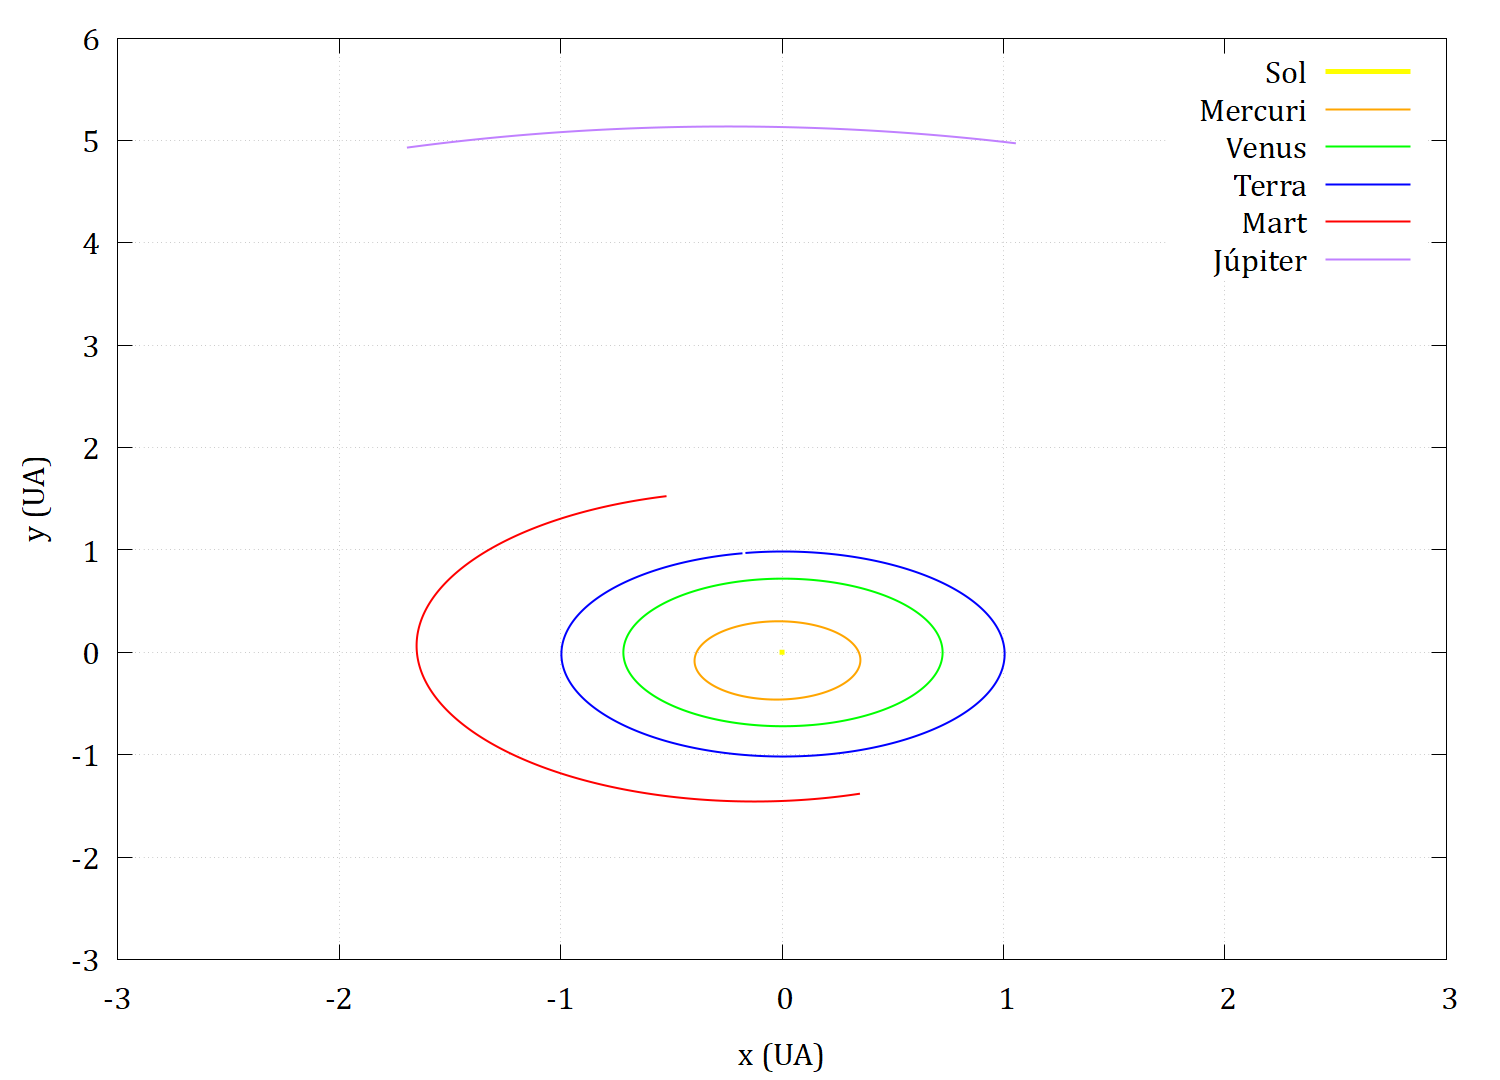
\includegraphics[width=\linewidth]{../sist_solar/orbites_euler_1_d1hora.png}
        \caption{Òrbites per $dt=1$ hora.}
        \label{fig:euler_implicit_solucio}
    \end{subfigure}
    \hfill
    \begin{subfigure}[b]{0.32\linewidth}
        \centering
        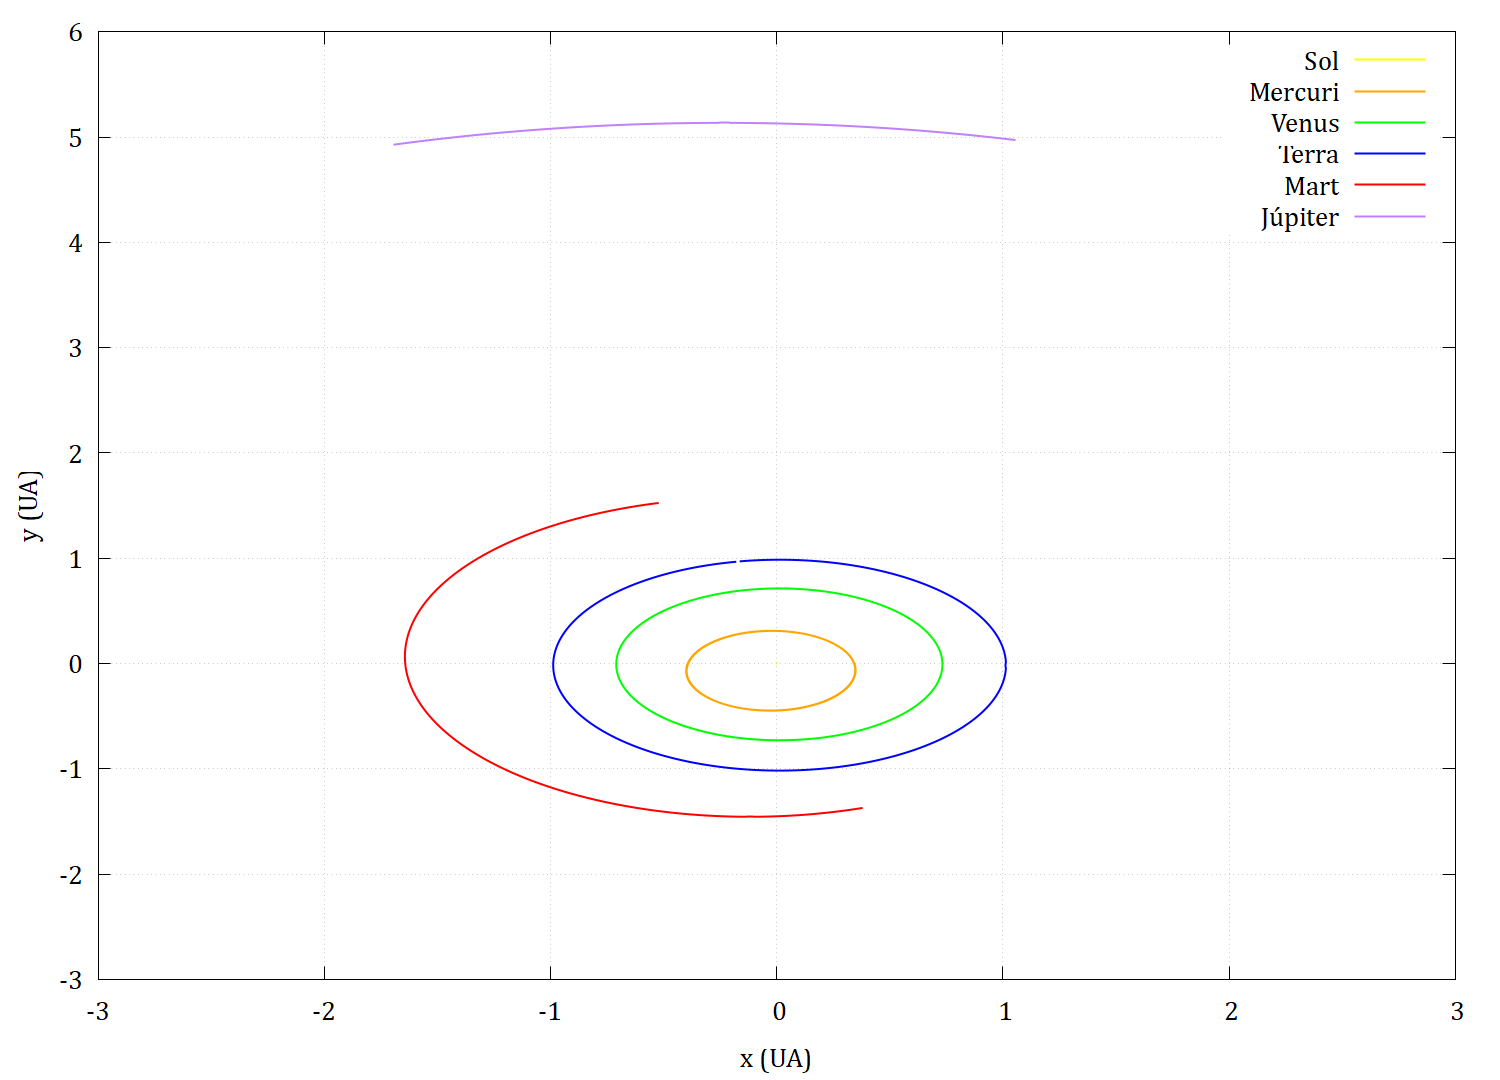
\includegraphics[width=\linewidth]{../sist_solar/orbites_euler_1_d1dia.png}
        \caption{Òrbites per $dt=1$ dia.}
        \label{fig:euler_implicit_errors}
    \end{subfigure}
    \hfill
    \begin{subfigure}[b]{0.32\linewidth}
        \centering
        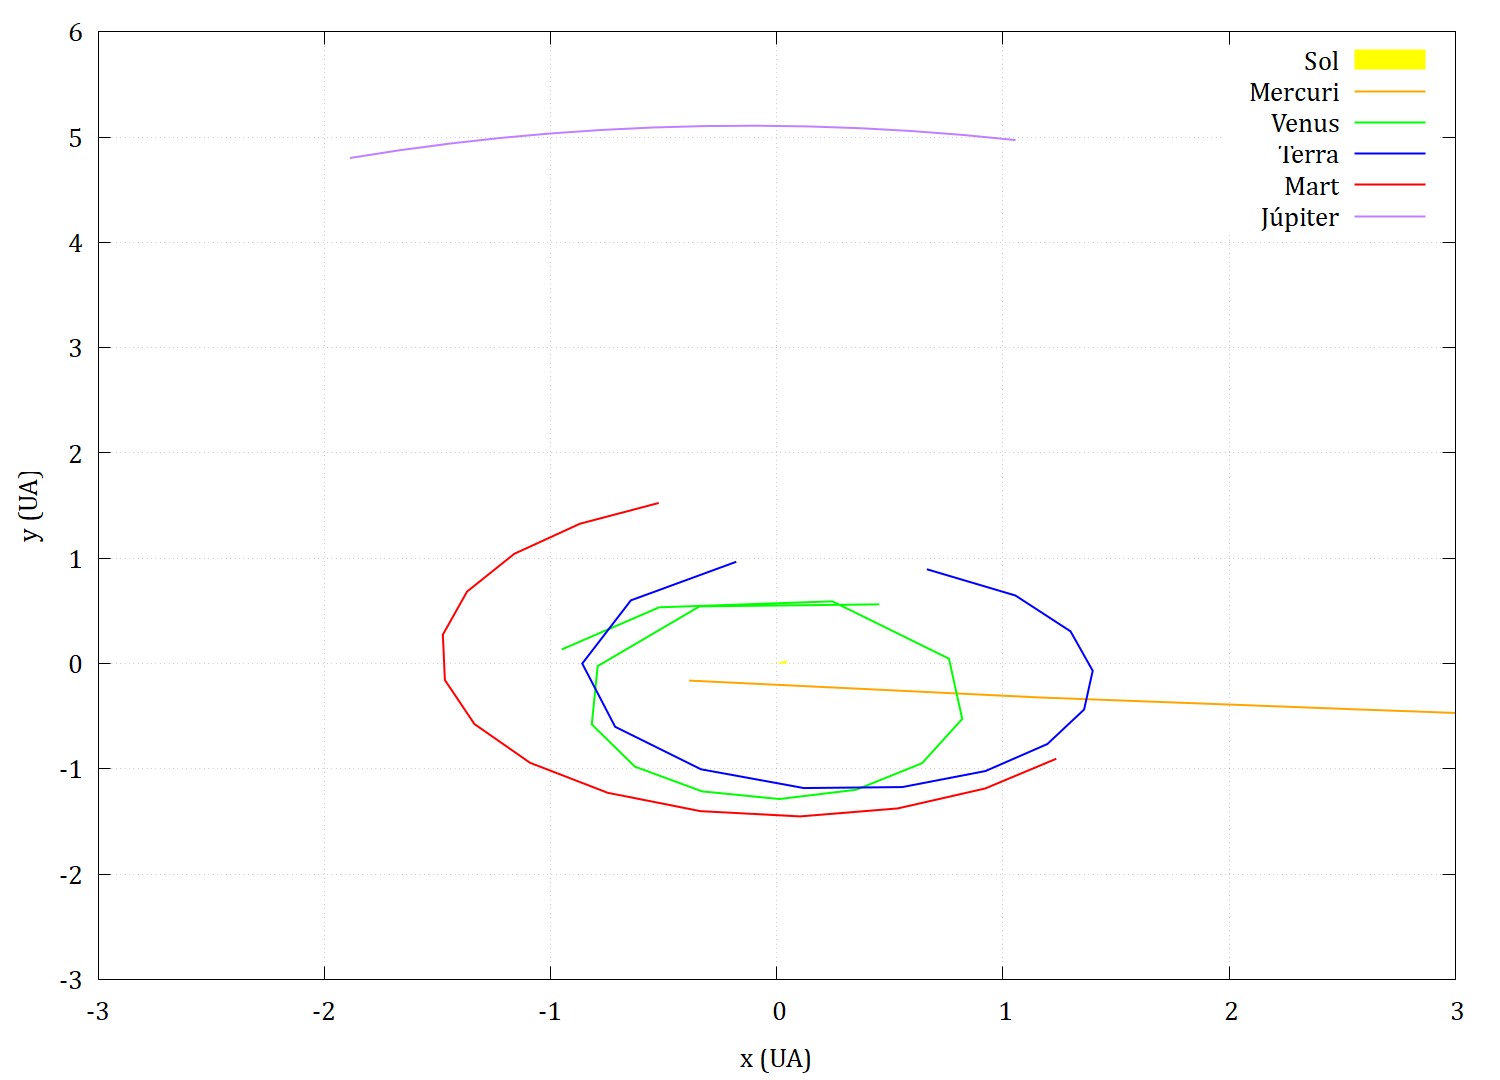
\includegraphics[width=\linewidth]{../sist_solar/orbites_euler_1_d1mes.png}
        \caption{Òrbites per $dt=1$ mes.}
        \label{fig:euler_implicit_errors}
    \end{subfigure}
    
    \caption{Òrbites del sistema solar a $t=1$ any (terrestre) per diferents valors de la discretització obtingudes.}
    \label{fig1}
\end{figure}

A l'annex \ref{an:a} podeu trobar les gràfiques corresponents a tot el Sistema Solar (amb els cossos no descrits aquí) i un seguit d'animacions per tal de visualitzar més clarament l'evolució temporal de tots els cossos fins a un $t_{final}=15$ anys.

Els errors relatius en l'energia associats als diferents planetes es poden veure a la figura \ref{fig3}

\begin{figure}[h!]
    \centering
    
    \begin{subfigure}[b]{0.32\linewidth}
        \centering
        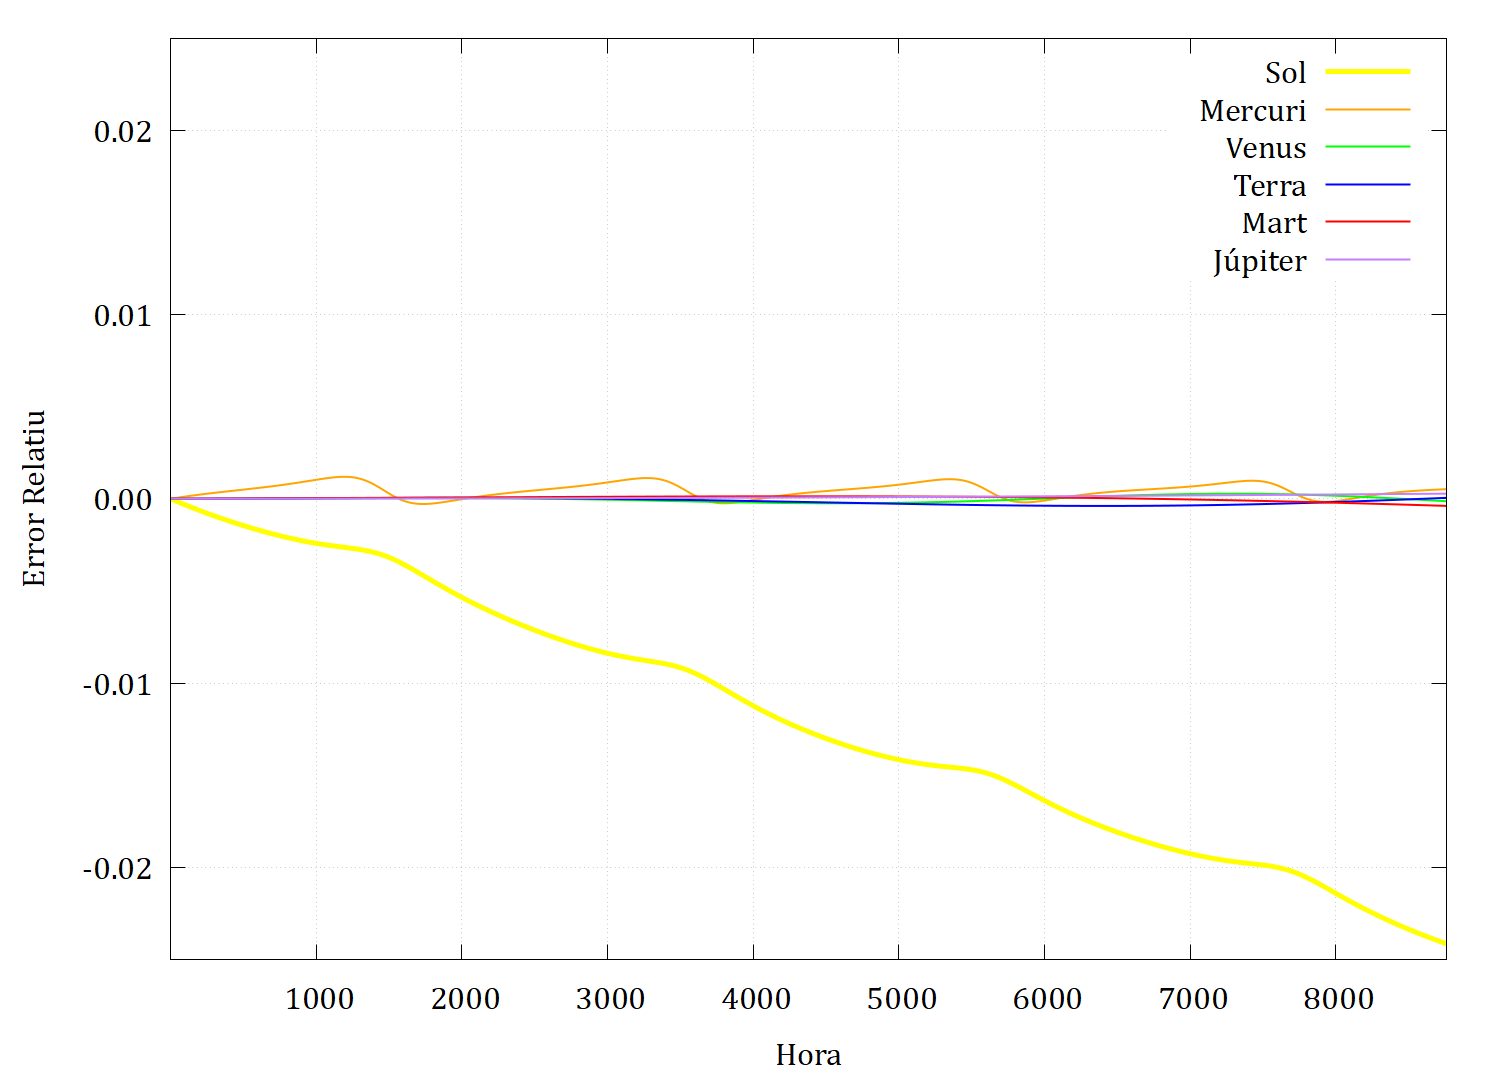
\includegraphics[width=\linewidth]{../Error/error_1_hora.png}
        \caption{Errors per $dt=1$ hora.}
    \end{subfigure}
    \hfill
    \begin{subfigure}[b]{0.32\linewidth}
        \centering
        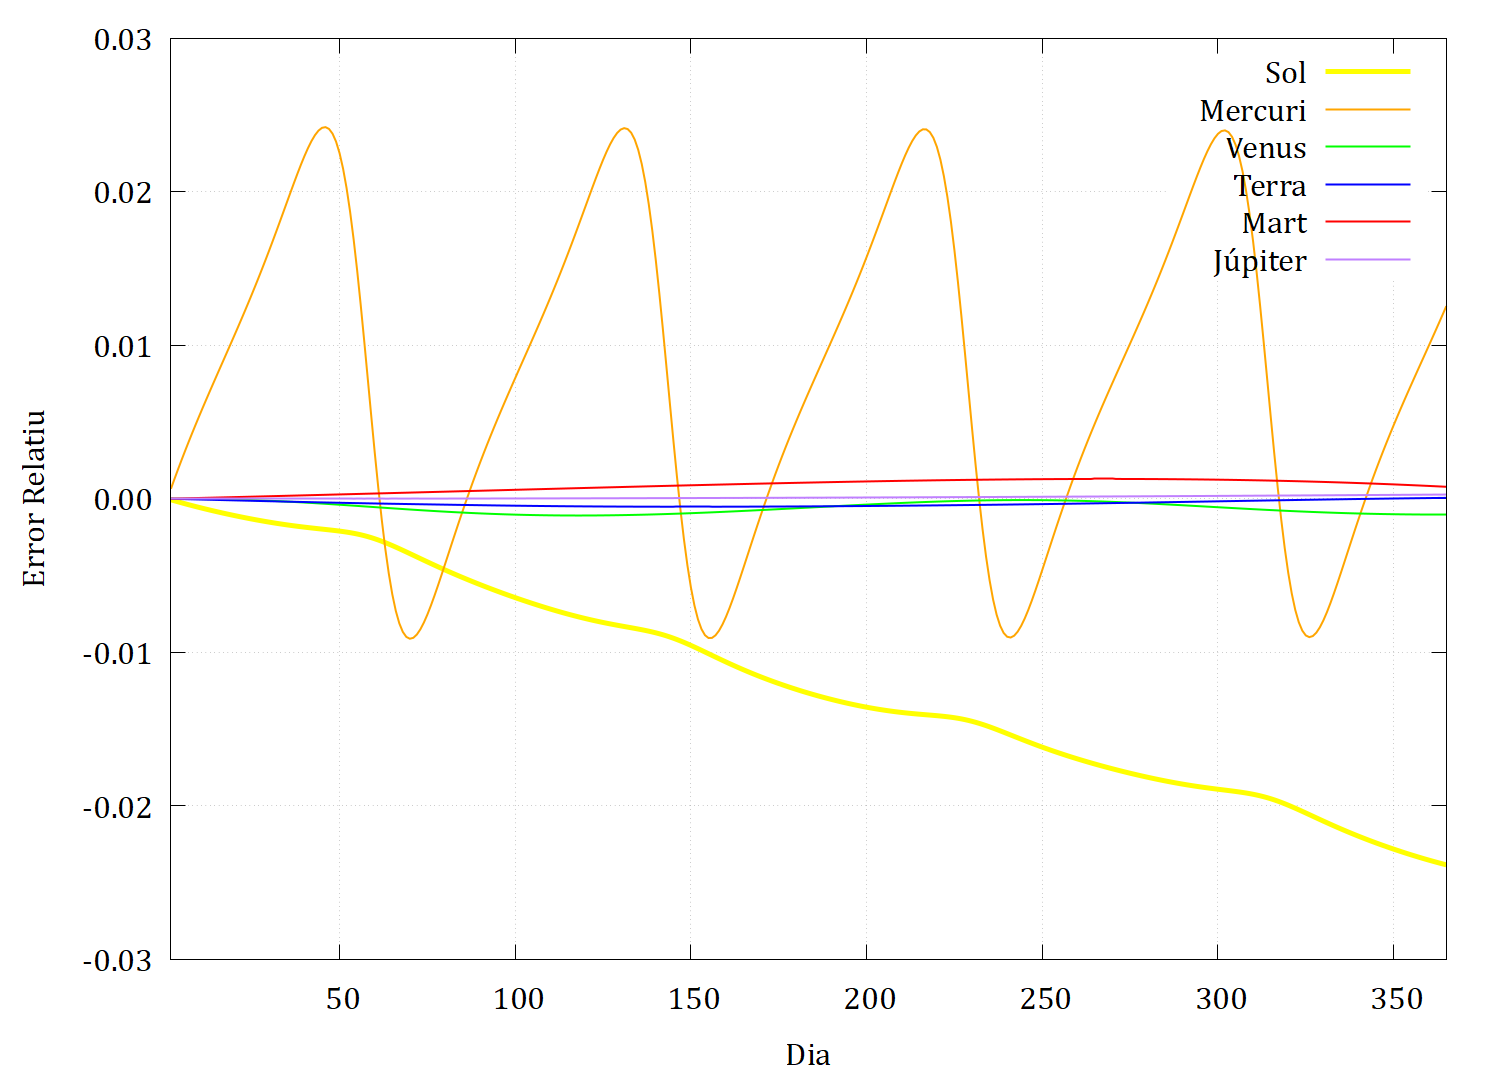
\includegraphics[width=\linewidth]{../Error/error_1_dia.png}
        \caption{Errors per $dt=1$ dia.}
    \end{subfigure}
    \hfill
    \begin{subfigure}[b]{0.32\linewidth}
        \centering
        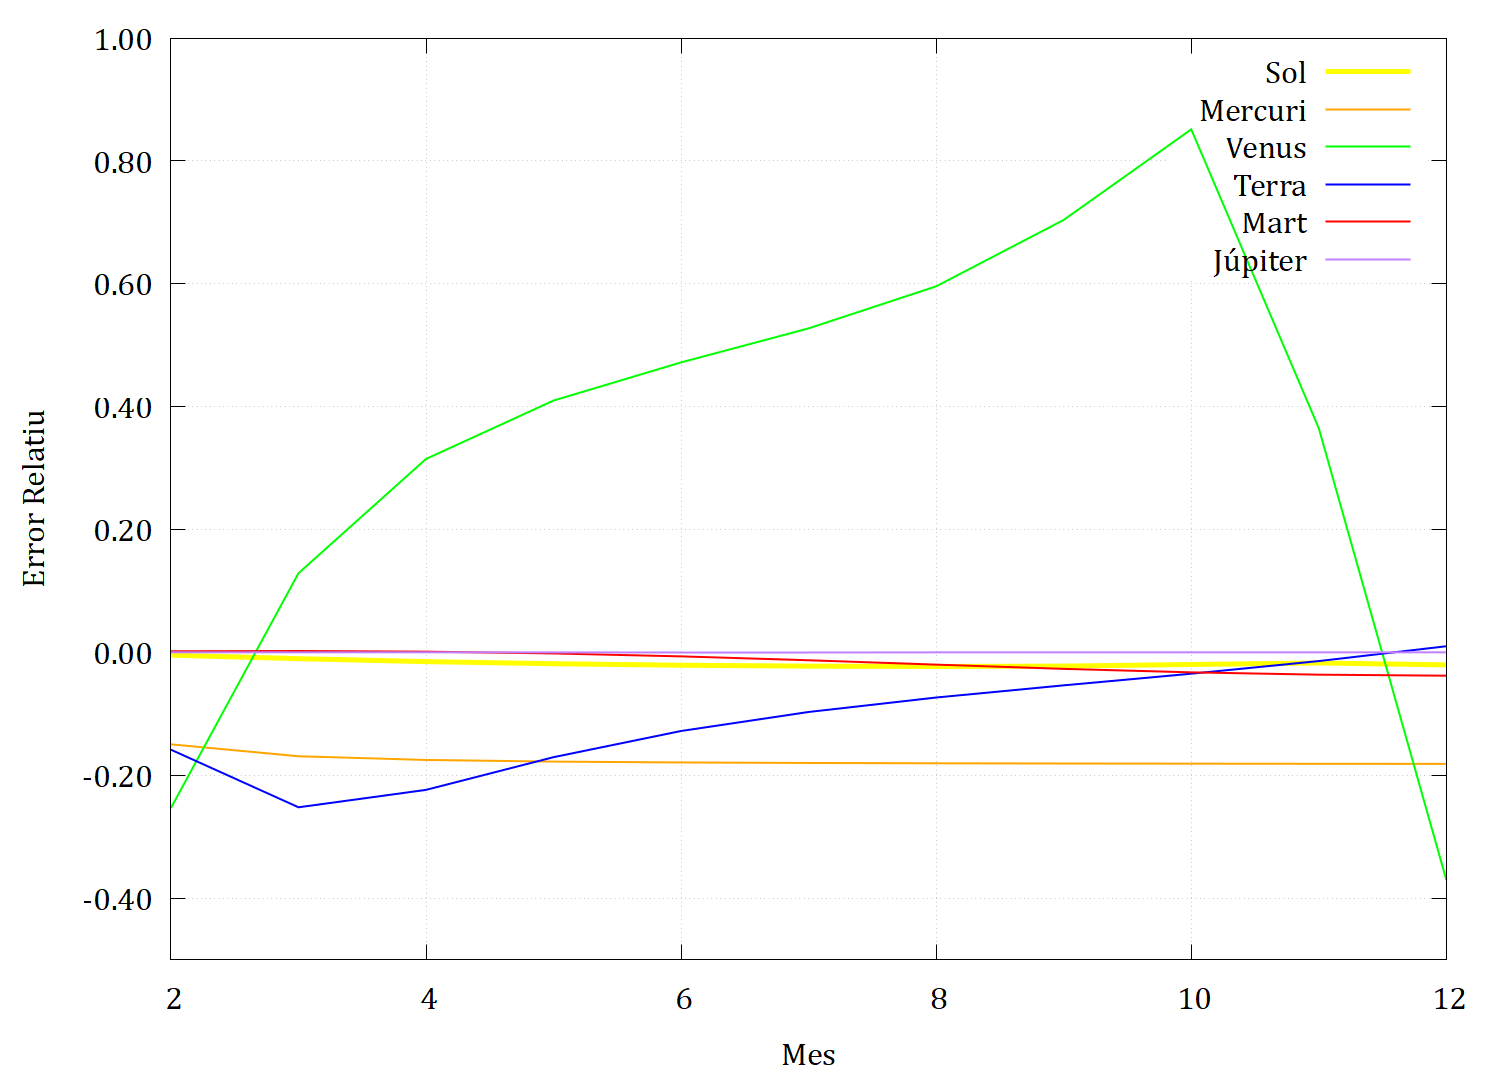
\includegraphics[width=\linewidth]{../Error/error_1_mes.png}
        \caption{Errors per $dt=1$ mes.}
    \end{subfigure}
    
    \caption{Errors relatius respecte l'energia inicial pels diferents cossos del Sistema Solar a partir de la solució trobada mitjançant el mètode d'Euler, classificat en funció de la discretització emprada, fins a $t_{final}=1$ any.}
    \label{fig3}
\end{figure}

Tal i com podem veure a les anteriors tres gràfiques, la discretització amb un major error numèric és la corresponent a $dt = 1$ mes, degut a que els grans salts en el temps fan que els errors asssociats al mètode d'Euler, que de per si no és molt bo, es disparin. En concret, podem veure com l'error associat a l'energia de Venus s'arriba a disparar fins a més d'un 80\%. La Terra i Mercuri tenen també errors relatius grans, sobretot al principi, essent aquests propers al 20\% (valor absolut). 

De fet, si ens fixem en la figura \ref{fig1}, per la discretització $dt=1$ mes, podem veure que Mercuri surt disparat del Sistema Solar. Que això no es vegi reflectit, aparentment, en l'error associat a l'energia de Mercuri (que es manté pràcticament constant en una desviació del 20\%) pot ser degut a què les variacions en els termes en l'energia cinètica i l'energia potencial d'aquest cos es compensen conforme l'astre s'allunya de la seva posició inicial.

Tant a la discretització de $dt = 1$ dia com a la de $dt = 1$ hora tenim errors associats als planetes més exteriors del sistema modelitzat similars, essent aquests lleugerament menors en el cas de la discretització per hores, a costa d'un temps de càlcul major. La principal diferència rau, però, en l'error associat a Mercuri: per a la discretització en dies presenta un error relatiu molt major al de la resta de cossos (exceptuant el Sol), assolint pics de fins a un 2.5\%; per a la discretització en hores aquest efecte es disminueix significativament.

Cal que comentem a part, però, el cas del Sol Per a les tres discretitzacions presenta una evolució de l'error associat a l'energia molt similar: en tots els casos té una clara tendència a desviar-se negativament. Podem explicar això si pensem en què el Sol és, dels 6 cossos modelitzats, el que ha tenir posicions i velocitats menors, de forma que l'acumulació d'errors associats al mètode numèric pot fer que aquestes petites quantitats es vegin afectades de forma significativa.

Si fem un estudi de l'evolució del Solar fins a un $t_{final}$ major, usant $dt=1$ dia, els resultats que s'obtenen són els que es poden veure a la figura \ref{fig4}.

\begin{figure}[h!]
    \centering
    \begin{subfigure}[b]{0.48\linewidth}
        \centering
        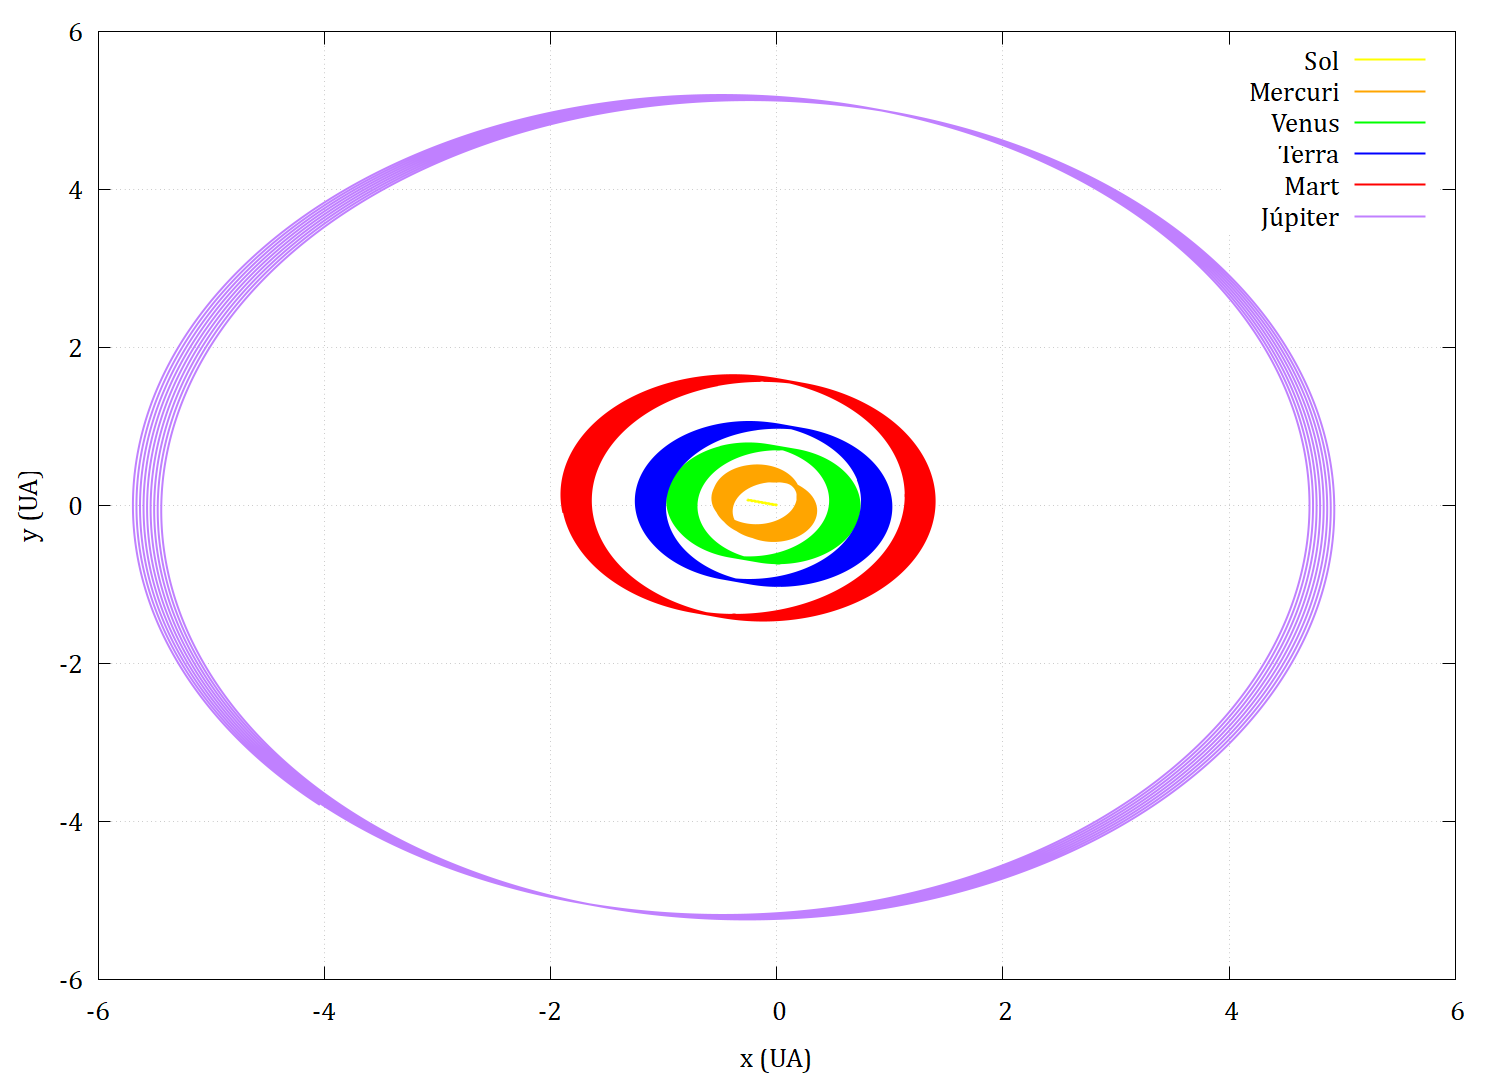
\includegraphics[width=\linewidth]{../sist_solar/orbites_euler_100_d1dia.png}
        \caption{Òrbites fins a $t_{final}=100$ anys amb $dt=1$ dia.}
    \end{subfigure}
    \hfill
    \begin{subfigure}[b]{0.48\linewidth}
        \centering
        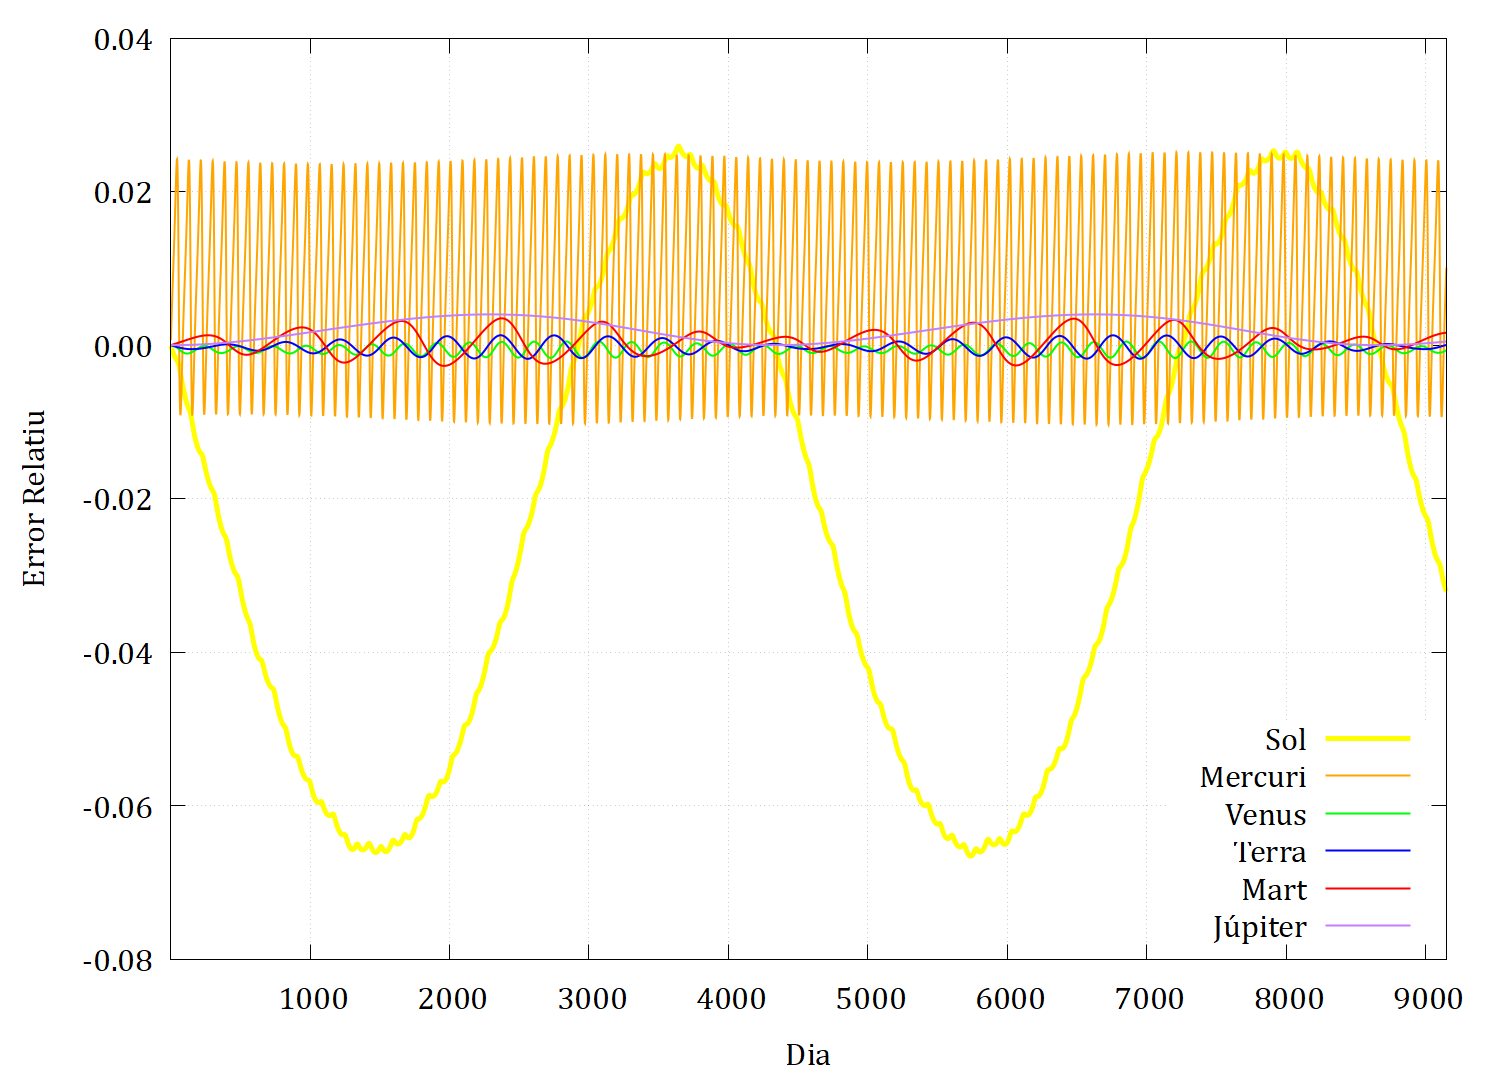
\includegraphics[width=\linewidth]{../Error/error_100_dia.png}
        \caption{Errors per $dt=1$ dia.}
    \end{subfigure}
    \caption{Estudi de l'evolució del Sistema Solar a $t_{final}$ major.}
    \label{fig4}
\end{figure}

Ara es posa de manifest el caràcter oscil·latori de l'error relatiu per tots els cossos del Sistema Solar. Podem veure com l'error màxim obtingut és proper al 6.5\% (valor absolut) en el cas del Sol, pels motius ja comentats abans\footnote{Per motius de qualitat, de la gràfica associada a l'error per $t_{final}=100$ anys arriba només fins als 50 anys. Podeu trobar més informació a l'enllaç de l'annex \ref{an:a}.}. La resta de planetes, exceptuant el cas de Mercuri, no arriben en cap cas a errors superiors al 1\%.

\subsection{Moviment del Sol sobre Mont-rós}
\textbf{(això s'ha de fer, gràfiques i tal)}

\subsection{Energia subministrada per la placa solar}
A les figures \ref{fig:figura1} i \ref{fig:figura2} es poden observar els histogrames corresponents a l'energia elèctrica generada cada mes al llarg d'un any de la nostra placa i la obtinguda a segons el model del PVGIS. 

\begin{figure}[h!]
    \centering
    \begin{minipage}{0.48\linewidth} 
        \centering
        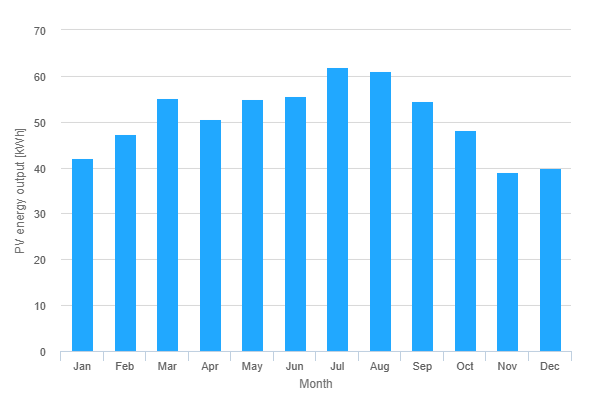
\includegraphics[width=\linewidth]{Histograma_PVGIS.png}
        \caption{Histograma de l'energia generada durant un any extreta de PVGIS}
        \label{fig:figura1}
    \end{minipage}\hfill 
    \begin{minipage}{0.48\linewidth} 
        \centering
        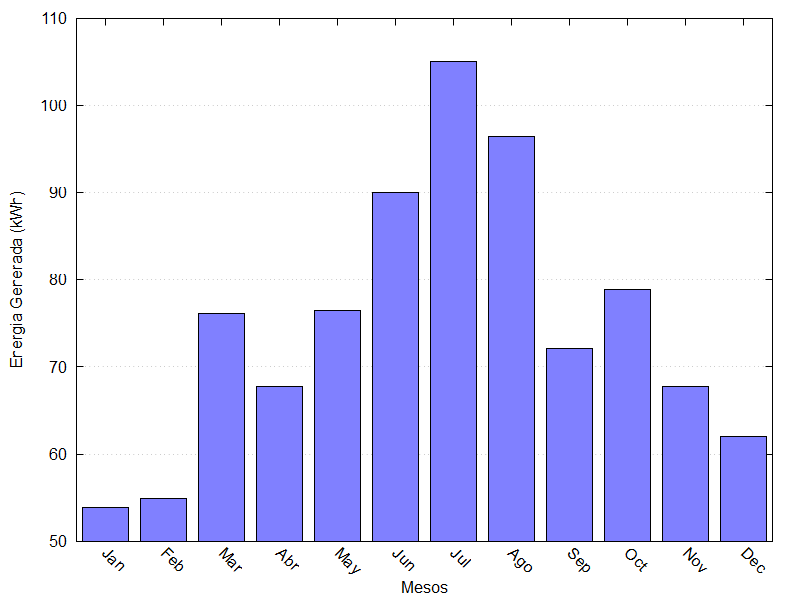
\includegraphics[width=\linewidth]{../Mov_sol/histograma.png}
        \caption{Histograma de l'energia generada durant un any del nostre model}
        \label{fig:figura2}
    \end{minipage}
\end{figure}


\textbf{(algun comentari per aquí)}

\section{Conclusions}

BLAHBLAHBLAH DEL SISTEMA SOLAR

\newpage
\begin{thebibliography}{99}
    \bibitem{ref1}
    Escartín, J.M. i Navau, C. \textit{Mètodes Numèrics II}. Apunts de l'Assignatura (veure CV).

    \bibitem{ref2}
    Aguilar, L. \textit{Modelizando el Sistema Solar}. Consultat el: 11/12/2024. \url{https://www.astrosen.unam.mx/~aguilar/MySite/Teaching_files/BasicEqns-1.pdf}.

    \bibitem{ref3}
    \textit{Horizon Ephemeris}, NASA. Web de consulta de les posicions de tots els astres del sistema solar. Consultat el: 23/12/2024. \url{https://ssd.jpl.nasa.gov/horizons/}.

    \bibitem{ref4}
    Universidad de Granada. \textit{El Sistema Solar y las Galaxias. Una Introducción a la Dinámica Molecular}. Consultat el: 11/12/2024. \url{https://ergodic.ugr.es/cphys/LECCIONES/ssolar/planetas-SLIDES.pdf}.

    \bibitem{ref5}
    \textit{MeteoGram}. Web per a consultar els horaris de les sortides i postes del Sol a tot el planeta. Consultat el: 05/01/2025. \url{https://meteogram.es/sol/espana/vielha/}.

    \bibitem{ref6}
    \textit{NASA Power}, NASA. Web per consultar la metereología de qualsevol lloc del món. Consultat el 07/01/2025. \url{https://power.larc.nasa.gov/data-access-viewer/}.

    \bibitem{ref7}
    \textit{Photovoltaic Geographical Information System (PVGIS)}. Web oficial de la Comissió Europea per a consultar informació sobre la radiació solar i sobre el rendiment i l'energia generada per plaques fotovoltaiques a qualsevol lloc del planeta (a excepció del Pol Nord i el Pol Sud). Consultat el 08/01/2025. \url{https://joint-research-centre.ec.europa.eu/photovoltaic-geographical-information-system-pvgis_en}.

    
\end{thebibliography}

\newpage
\appendix
{\Huge{\textbf{Annexos}}}
\section{Repositori de \textit{GitHub}}
\label{an:a}
Podeu trobar els codis usats en \textit{Fortran}, les representacions de les gràfiques usant \textit{Gnuplot}, animacions de les simulacions del sistema solar i més al següent repositori (públic) de \textit{GitHub}: \url{https://github.com/elitus7/PSimulacio_MN2}.

\section{Simulació del Sistema Solar amb més cossos}
\label{an:b}
A mode d'extra, afegim en aquest annex els resultats de la simulació del Sistema Solar considerant també Saturn, Urà i Neptú (més enllà dels cossos del model del text principal) mantenint, però, la condició que el moviment es dóna en un únic pla. A la figura \ref{fig:an1} podeu veure les òrbites obtingudes usant una discretització de $dt=1$ dia, que com hem vist és la millor pel que fa a temps de càlcul i exactitud, i un $t_{final}=150$ anys.

\begin{figure}[h]
    \centering
    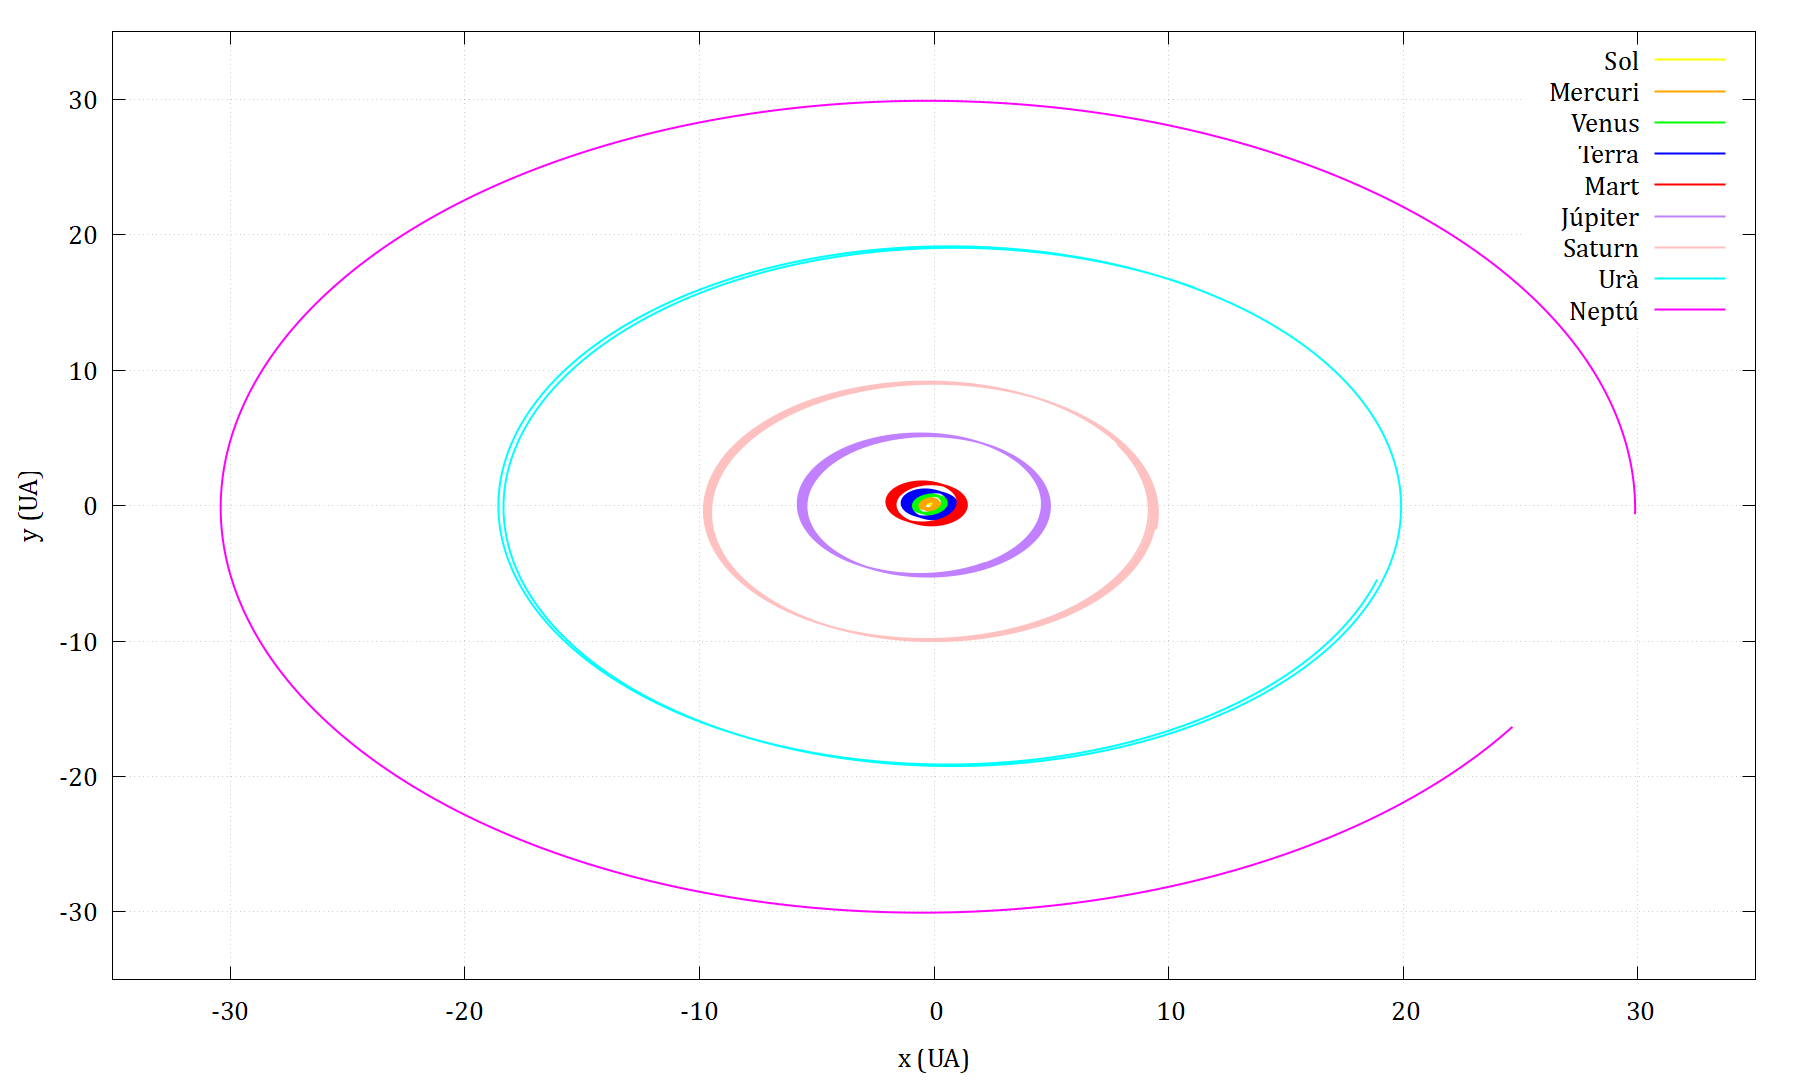
\includegraphics[width=1.0\linewidth]{../sist_solar/orbites_euler_TOTS_150_d1dia.png}
    \caption{Òrbites obtingudes amb el mètode d'Euler per a una simulació amb $dt=1$ any fins a $t_{final}=150$ anys per tots els cossos importants del Sistema Solar.}
    \label{fig:an1}
\end{figure}

Al repositori de \textit{GitHub} podreu veure una animació, a $t_{final}=15$ anys, en la que es poden veure les òrbites anteriors.
\end{document}